\section{Introduction}
\label{sec:intro}

Supporting sequences (arrays) with efficient (constant time)
accesses and updates has been a persistent problem in functional languages
(pun not intended).  It is easy to implement such sequences with constant
time random access reads (using arrays stored as contiguous memory),
or to implement with logarithmic time reads and updates using balanced
trees, but it seems that getting both in constant time cannot be
achieved without some
form of extension.
%~\cite{Pippenger97}.  
This means that algorithms
for many fundamental problems are a logarithmic factor slower in
functional languages than in imperative languages.  This includes
algorithms for basic problems such as generating a random permutation,
and for many important graph problems (e.g.,
shortest-unweighted-paths, connected components, biconnected
components, topological sort, and cycle detection).  Simple algorithms
for these problems take linear time in the imperative setting, but an
additional logarithmic factor in time in the functional setting, at
least without extensions.

A variety of approaches have been suggested to alleviate this problem.
Many of the approaches are based on the observation that if there is
only a single reference to an array, it can be safely updated in
place.  The most common such approach is to use
monads~\cite{Moggi89,Wadler95}.  Monads can force code to be single
threaded and can thread mutable arrays (or other mutable
state) so the only reference to them is the current one.
Haskell supplies the ST monad for this purpose.  King and Launchbery,
for example, use STMonads with an array to implement depth first 
search (DFS) in linear work~\cite{KL95}.  Guzman and Hudak's single-threaded
lambda calculus also uses the idea of single threading the
computation~\cite{GH90}, and they motivate the approach based on allowing
for fast array updates.  The problem with using these approaches is
that they are basically implementing a second imperative language within
a functional language.  Using monads means using a new syntax not just
for the operations themselves but for much of the code the operations are
embedded in.  Indeed King and Launchbery have to write completely
different code for DFS, even though it is only for efficiency and not
correctness (it is trivial to implement DFS in $O(m \log n)$ time
purely functionally).  Monads also do not allow keeping persistent
versions of structures, exactly because the state can be changed.
More importantly, however, monads force the program itself to be single
threaded, inhibiting parallelism.

A second approach is to use a type system that enforces the
single-threadedness of individual arrays rather than the program as a
whole.  This can be done with linear types~\cite{Girard87,Wadler90},
which can be used to ensure that references are not duplicated.  This
is more flexible than monads, since it allows the threading of the
data to be distinct from the threading of the program.  However, such
type systems are not available in most languages, and they can be hard
to reason about.   

A third approach is to support fully functional arrays in a general
functional language, and to check either statically or dynamically if they happen to be
used in a single threaded manner.  This can be done, for example, by
using reference counting~\cite{HB85,Hudak86}.  The idea is to keep
track of how many references there are to an array and update in place
if there is only one.  Hudak describes techniques to statically
analyze code to determine that at certain points in the code a count
must be one, and therefore it is safe to replace an update with an
in place update.  The problem with this approach is that the efficiency
of the code depends heavily on the effectiveness of the compiler and
the specific way the code is written, and it can therefore be hard for
the user to reason about efficiency.

The last approach is to fully support functional arrays, even with
sharing, but using more sophisticated data structures.  This is
sometimes referred to as version tree arrays~\cite{AHN88} or fully
persistent arrays~\cite{DSST89}. The idea is to maintain a version
tree for an array (or more generally other data types), such that any
node of the tree can be updated to create a new leaf below it with the
modified value, without effecting the value of other nodes.  Dietz
showed that arrays can be maintained fully persistently using
$O(\log\log n)$ time per operation (read or write).  Holmstrom, Hughes
and others (see \cite{AHN88}) suggested storing a version tree by
keeping the full array at the root, and a each node represents an
update.  Chuang's approach ~\cite{chuang} supports $O(1)$ accesses and
insertions to the most recent version of arrays, however accessing old
versions of the array takes $O(n)$ work which is often impractical.
O'Neill and Warren~\cite{oneill} describe various improvements.
The problem with these approaches is that they can be very complicated,
and only efficient in certain cases. Furthermore it can be hard to
reason about the performance.

None of the existing approaches properly support concurrent operations on
functional arrays.  O' Neill suggests (in passing) having a lock for each element
of the array. However, when many threads contend for the same element,
this would serialize accesses and therefore they would not take
constant time.   Additionally, per-element locks add significant memory
overhead.  

% Using arrays in a concurrent or persistent manner is not simply of theoretical importance. As an example application, consider a producer-consumer situation where a producer is rapidly writing values to a mutable array and a consumer has registered a callback that triggers when the array reaches a certain state. The callback expects to see what the array was like when the event was triggered, even though the producer may continue writing values to the array. The naive way to implement this is to copy the array and pass the copy to the callback. However, copying the array is inefficient and the producer is blocked from making progress during the copy. We can use concurrent functional arrays for this application.

% Separation logic ~\cite{reynolds} could be used to
% parallelize divide and conquer algorithms on arrays however they would
% severely restrict the way functional arrays can be used.

\subsection*{Our Approach: Sequences}

In this paper we present an approach for efficiently supporting
functional arrays (sequences).  It uses some ideas from the previous approaches
but unlike the previous approaches it supplies a well
defined cost dynamics, and supports parallelism, and without language
extensions.  More specifically the approach has the
following important features.
\begin{enumerate}
\item It has fully functional value dynamics---i.e., when not considering costs, sequences act no
  differently than purely functional sequences.
\item It requires no changes in existing languages and no special
  types, syntactic extensions, etc.  Programs can be efficient---i.e.,
  constant time reads and writes---when using a completely standard
  functional programming style.
\item The approach supports nested parallelism---sequences can be passed
  to parallel calls and safely updated and read, again with a purely
  functional dynamics.
\item We supply a well defined cost dynamics, which can be used to
  formally analyze the cost of any program.  The dynamics captures
  both sequential and parallel costs.
\item We describe a cost-bounded implementation which maps costs in the
  model to costs on either a sequential or parallel RAM (PRAM).
\item
Although accessing old versions of a sequence is more expensive than
accessing new versions (as defined in the cost dynamics), reading old
versions never costs more than $O(\log n)$ work.
\end{enumerate}
We have implemented the approach and in this paper present some
performance numbers.

Although our value dynamics is purely functional (and compositional)
our cost dynamics is not---they require passing a store and modeling
costs based on the order the store is threaded.  To allow for
parallelism we allow for arbitrary interleaving of the steps in the
cost dynamics.  We note that lazy languages also have a pure value
%dynamics but impure cost dynamics---call-by-name and call-by-value
dynamics but impure cost dynamics---call-by-name and call-by-need
only differ in their costs, and a store is required to model the
difference~\cite{AMOFW95}.

\begin{figure}[!ht]
\centering 
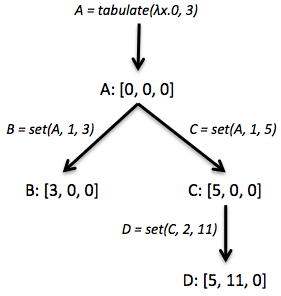
\includegraphics[scale=0.45]{leaf_interior_intro}
\nocaptionrule \caption{Example usage of sequences}
\label{fig:leaf_interior_intro}
\end{figure}

In this paper we consider sequences with three functions: \new{},
\get{} (read), and \set{} (write). \new{}$(n,v)$
creates a new sequence of length $n$ with the value $v$ at each index, \get$(A,i)$ returns the $i$-th element of $A$, and
\set$(A,i,v)$ returns a ``new'' sequence where the $i^{th}$ element of $A$ is replaced by $v$ (in the following discussion $n$ refers to the length of
an sequence).  Figure~\ref{fig:leaf_interior_intro} gives an example.  

As in previous work~\cite{AHN88} the history of a sequence after it is
created with \new{} can be viewed as a version tree.  A version
tree has interior nodes and leaves.  In the figure, after all
functions are applied, sequences $A$ and $C$ are \emph{interior nodes},
and sequences $B$ and $D$ are \emph{leaves} of the version tree.  In our
cost dynamics applying \get{} and \set{} to sequences at the leafs takes
constant work, but applying them to interior nodes is more expensive.

We start with a simple pure call-by-value lamba calculus extended with
sequences.  To define abstract costs and show the relationship to
concrete cost (time) on a parallel machine we use two levels of cost
dynamics: a structural cost dynamics and a evaluation cost dynamics.
Our structural cost dynamics is a single step dynamics and is closer
to the implementation.   The dynamics defines the work by summing the
cost per transition across an arbitrary interleaving of the potential transitions
(due to concurrency), and defines the span by allowing all potentially
parallel transitions to proceed together.    We prove a mapping of the
cost in the structural dynamics to time on a $P$ processor machine,
assuming given costs for the sequence functions.   The cost is
non-deterministic due to different possible interleavings.

The evaluation dynamics is a higher-level big-step dynamics more
appropriate for a programmer to reason about costs.  In particular the
costs in the evaluation dynamics are deterministic independent of
interleaving.  We prove that the costs in the evaluation dynamics
gives a tight worst case upper bound on the cost of the underlying structural
dynamics, allowing for any interleaving.

We describe the implementation in an impure language---our pure
language extended with references and an atomic compare-and-swap on
those references.  To implement sequences, we maintain at
each leaf of the version tree a mutable array of the most recent values.  We
also keep with each location a change-log that keeps track of values
at interior nodes of the version tree.  Applying \get{} to a leaf only
requires a lookup in the array.  Applying \set{} to a leaf only
requires updating the array, and adding an element to the change log
for the old version.  Applying \get{} to an interior nodes requires a
binary search on the change log, which can be bounded by $O(\log n)$
time.  To ensure that change logs do not get too large, whenever the
total size across all change logs reaches $n$, the array is copied.
This requires $O(n)$ time, but can be amortized against the updates.
Applying \set{} to an interior node requires creating a new array, and
copying values to it.  This requires $O(n)$ time.

We give a wait-free concurrent implementation that uses careful
synchronization.   We assume that instructions in the target language
can be interleaved in any way--i.e., at any given step many \get{}s and
\set{}s can be in progress.   All we require is that memory reads,
writes and compare-and-swap are atomic.  We show correctness with
respect to any interleaving, and show that specific linearization
points within the implementation define the relative order of \get{}s
and \set{}s with respect to the structural dynamics.

To evaluate our approach in practice we ran a variety of experiments
on a preliminary concrete implementation.  The
experiments show that accesses are $3\%$ to $12\%$ slower in leaf sequences
than in regular Java arrays, and updates are $2.4$ to $3.3$ times slower.
Considering the purity and additional functionality provided by our sequence
implementation, this is a small slowdown. Furthermore, preliminary experiments 
back up our theoretical claim that threads can access our sequences with a high 
level of concurrency.

Our results on cost dynamics can be easily extended to other data
types where the cost of \get{} and \set{} are different for leaf and
interior versions, even if there are multiple varieties of \get{} and
\set{} functions.   In particular, our sequence implementation can likely
be extended to functional unordered sets implemented with hash tables,
and our approach might be useful in coming up with more efficient
implementations of functional disjoint sets (although a functional
disjoint set implementation where all operations cost $\log{n}$ is
known~\cite{persistentufds}).
